\section{Reduced Cross Section}

The experimental cross section is given by equation \ref{xsec}

 \begin{equation}\label{xsec}
     \frac{d^4\sigma_{\gamma^*p \rightarrow p'\pi^0}}{dQ^2dx_Bdtd\phi_{\pi}} = \frac{N(Q^2,x_B,t,\phi_{\pi})}{\Lumi_{int}\Delta Q^2\Delta x_B\Delta t\Delta \phi} \frac{1}{\epsilon_{ACC} \delta_{RC} \delta_{Norm} Br(\pi^0 \rightarrow \gamma \gamma)}
\end{equation}

$N(Q^2,x_B,t,\phi_{\pi})$ is the raw number of events in a specific kinematic bin and is calculated as described in chapter \ref{Chapter:BaseAnalysis}. $\Lumi_{int}$ is the integrated luminosity over the run of the experiment under analysis and is calculated as described in chapter \ref{sec:luminosity}.$\Delta Q^2\Delta x_B\Delta t\Delta \phi$ are the bin widths for the 4 kinematic binning variables. $\epsilon_{ACC}$ is the acceptance correction, and is calculated as described in chapter \ref{Chapter:BaseAnalysis}. $\delta_{RC} \delta_{Norm} Br(\pi^0 \rightarrow \gamma \gamma)$ are the radiative, overall, and branching ratio correction factors, and are not yet included in this cross section calculation. 
\\~\\
Initial investigations show that radiative corrections will be on the order of 5\%, the branching ratio is a 1.2\% correction, and the overall normalization is not yet determined but was 10\% for the CLAS6 experiment; we expect the CLAS12 experiment overall normalization will be similar or less in magnitude. Thus, all of these corrections are much smaller than the acceptance correction, and will be included in future work but are not critical for preliminary analysis work.

The accepted results from the CLAS6 experiment \cite{Bedlinskiy2014ExclusiveCLAS} can be used as a cross check for this work. Published values for the reduced cross sections from the CLAS6 experiment for the DV$\pi^0$P channel are available \href{https://journals.aps.org/prc/supplemental/10.1103/PhysRevC.90.025205}{here}. To calculate the reduced cross sections, we divide the cross section as described in equation \ref{xsec} by the virtual photon flux factor $\Gamma$ for each kinematic bin, where $\Gamma$ is calculated as described in chapter \ref{sec:luminosity}. The reduced cross section is then given by equation \ref{eq:basic_xsec}.

 \begin{equation}\label{xsec_red}
    \frac{d^2\sigma_{\gamma^*p \rightarrow p'\pi^0}(Q^2,x_B,t,\phi_{\pi},E)}{dtd\phi} = \frac{1}{\Gamma_V(Q^2,x_B,E)} \frac{d^4\sigma_{\gamma^*p \rightarrow p'\pi^0}}{dQ^2dx_Bdtd\phi_{\pi}}
\end{equation}


 \begin{equation}\label{xsec_red_full}
    \frac{d^2\sigma_{\gamma^*p \rightarrow p'\pi^0}}{dtd\phi} = \frac{1}{\Gamma_V(Q^2,x_B,E)} \frac{N(Q^2,x_B,t,\phi_{\pi})}{\Lumi_{int}\Delta Q^2\Delta x_B\Delta t\Delta \phi} \frac{1}{\epsilon_{ACC} \delta_{RC} \delta_{Norm} Br(\pi^0 \rightarrow \gamma \gamma)}
\end{equation}
Some plots of reduced cross section for CLAS12 outbending Fall 2018 dataset are shown in figure \ref{fig:reduced_xsec_plots}. The cross sections show good agreement with the published CLAS6 results. The outbending dataset is contains mostly lower $Q^2$ events and the inbending dataset is not yet properly analyzed, so higher $Q^2$ comparisons are not avaliable for this analysis note. 


\begin{figure}[hbt]
	\centering
	\includegraphics[page=125,width=0.3\linewidth]{Chapters/Ch5-FurtherAnalysis/reduced_xsecs/ReducedCrossSectionFitOverPhi_Q2175_x_B022_t03.png}
	\includegraphics[page=123,width=0.3\linewidth]{Chapters/Ch5-FurtherAnalysis/reduced_xsecs/ReducedCrossSectionFitOverPhi_Q2175_x_B022_t12.png}
	\includegraphics[page=128,width=0.3\linewidth]{Chapters/Ch5-FurtherAnalysis/reduced_xsecs/ReducedCrossSectionFitOverPhi_Q2175_x_B022_t17.png}
	\includegraphics[page=130,width=0.3\linewidth]{Chapters/Ch5-FurtherAnalysis/reduced_xsecs/ReducedCrossSectionFitOverPhi_Q2138_x_B017_t12.png}
	\includegraphics[page=133,width=0.3\linewidth]{Chapters/Ch5-FurtherAnalysis/reduced_xsecs/ReducedCrossSectionFitOverPhi_Q2187_x_B027_t05.png}
	\includegraphics[page=135,width=0.3\linewidth]{Chapters/Ch5-FurtherAnalysis/reduced_xsecs/ReducedCrossSectionFitOverPhi_Q2195_x_B031_t05.png}
	
	\caption{Comparison of CLAS12 (blue) and CLAS6 (red) reduced cross sections, using Fall 2018 outbending dataset. Error bars are statistical only.}
	\label{fig:reduced_xsec_plots}
\end{figure}

To compare these results, we can examine the form of the differential cross section, under the single photon exchange assumption we can write the differential cross section as in equation \ref{eq:basic_diff_xsec}

 \begin{equation}\label{dif1}
     \frac{d^4\sigma_{\gamma^*p \rightarrow p'\pi^0}}{dQ^2dx_Bdtd\phi_{\pi}} =
     \Gamma (Q^2, x_B, E)
     \frac{1}{2\pi}
     ((\frac{d\sigma_T}{dt}+\epsilon\frac{d\sigma_L}{dt})+
     \epsilon cos(2\phi) \frac{d\sigma_{TT}}{dt} + \sqrt{2\epsilon(1+\epsilon)}cos(\phi)\frac{d\sigma_{LT}}{dt})
\end{equation}

Where $\Gamma (Q^2, x_B, E)$ is the virtual photon flux, give in equation \ref{gamma1}
 \begin{equation}\label{gamma1}
            \Gamma (Q^2, x_B, E) = \frac{\alpha}{8\pi} \frac{Q^2}{m^2_pE^2}\frac{1-x_B}{x_B^3}\frac{1}{1-\epsilon}
\end{equation}

The reduced cross section terms then are just functions of the structure functions and epsilon. At these kinematics, epsilon is approximately 0.5 for the CLAS6 data and 0.9 for the CLAS12 datasets, but given that the $((\frac{d\sigma_T}{dt}+\epsilon\frac{d\sigma_L}{dt})$ dominates the cross section, these differences are minor. Therefore, close (but not exact) agreement between the two datasets for given kinematic bins are expected for the reduced cross sections. More quantitative statements will be made in coming months, but not at this point.


\section{T Dependence of Cross Section}

We can calculate the t dependence of the differential cross section $d\sigma_U/dt$ by integrating the reduced cross sections over $\phi$ as in equation \ref{eq:tdep}

 \begin{equation}\label{eq:tdep}
    \frac{d\sigma_U}{dt} = \int \frac{d^2\sigma}{dtd\phi} d\phi
\end{equation}

In order to account for regions where the detectors used in CLAS6 and CLAS12 have zero acceptance, it is necessary to include a correction factor $\eta'$, defined in equation \ref{eq:eta} and calculated using Monte Carlo. 

 \begin{equation}\label{eq:eta}
    \eta' = \frac{\int_{\Omega*} \frac{d^2\sigma}{dtd\phi} }{\int_{\Omega} \frac{d^2\sigma}{dtd\phi}}
\end{equation}

However, at this point this correction factor has not yet been calculated. Instead, we can focus on kinematic bins where the coverage in $\phi$ is nearly 100\%, such that $\eta'$ would be small. In figure \ref{fig:tdep} we show the t dependent cross section, calculated only for bins where the coverage in $\phi$ was greater than 90\%, thus the error from not including the $\eta'$ correction factor is only approximately 10\%. We observe a good agreement in the b slope parameter, which describes the width of the transverse momentum distribution of the proton, between CLAS12 and the published CLAS6 data.


\begin{figure}[hbt]
	\centering
	\includegraphics[page=125,width=0.45\linewidth]{Chapters/Ch5-FurtherAnalysis/tdep/fig_1.0_0.15.png}
	\includegraphics[page=130,width=0.45\linewidth]{Chapters/Ch5-FurtherAnalysis/tdep/fig_1.5_0.15.png}

	\caption{CLAS12 and CLAS6 t dependence of cross sections. The fits are exponential functions $Ae^{-bt}$, where the slope parameter b are in close agreement for the bins considered. The overall normalization A is not yet determined for the CLAS12 dataset, so a small overall offset from the CLAS6 data is expected. Errors are only statistical.}
	\label{fig:tdep}
\end{figure}
